\documentclass{beamer}
\usepackage{beamerthemesplit}
\usepackage{graphics}
\usepackage[noend]{algorithm2e}
\usepackage{amsmath}
\usepackage{amssymb}
\usepackage{listings}
\usepackage{tikz}
\usepackage{soul}
\usepackage{mathtools}
\newtheorem{thm}{Theorem}


\DeclarePairedDelimiter\abs{\lvert}{\rvert}%
%\usepackage{algorithm}
%\usepackage{algorithmic}
\lstset{
basicstyle=\small,
keywordstyle=\color{blue}\bfseries,
numbers=left,
numberstyle=\tiny,
numbersep=5pt,
showstringspaces=false,
showspaces=false,
captionpos=b,
frame=tb,
float=tbh,
,escapeinside={*@}{@*}
}
%\usetheme{Boadilla}
\title{Algorithm Design}
\subtitle{Dynamic Programming}
\author{Hikmat Farhat}
%\email{hfarhat@ndu.edu.lb}
%\institution{Notre Dame University}
\newtheorem{mydef}{Definition}
\newtheorem{lem}{Lemma}
%\newcommand{\emphasis}[1]{\textcolor{yellow}{#1}}
%\newcommand{\emphasis}[1]{\hl{#1}}
\newcommand{\emphasis}[1]{\ul{#1}}
\newcommand{\floor}[1]{\lfloor{#1}\rfloor}
\newcommand{\bfloor}[1]{\Big\lfloor{#1}\Big\rfloor}
\newcommand{\modulus}[1]{\ensuremath\mid\!\!{#1}\!\!\mid}
%\newcommand{\gets}{\ensuremath{\leftarrow}}
%\DeclareTextFontCommand{\emph}{\emphasis}
\sethlcolor{yellow}

\begin{document}
\date{}

\frame{\titlepage}

\section{Independent Set}
\begin{frame}
  \frametitle{Independent Set (Linear)}
  \begin{itemize}
  \item Given a graph $G=(V,E)$ an independent set is a subset of vertices $S\subseteq V$ such that for all $x,y\in S$, $(x,y)\notin E$.
  \item Usually we need to an independent set such that $|S|$ is maximum. This general problem is hard to solve in the general case(see NP chapter later)
  \item In this lecture we consider a special case of the independent set: when all vertices are on the same line.
  \item The solution for this particular case is trivial: select every other node.
 \item We make things interesting by adding a weight to each node and asking : what is the independent set which has the largest total weight?
  \end{itemize}
\end{frame}

\begin{frame}
  \frametitle{Example}
  \begin{itemize}
  \item An example of the (linear) independent set problem with weights is shown below. Clearly the solution in this case is $\{x_2,x_4\}$.
  \end{itemize}
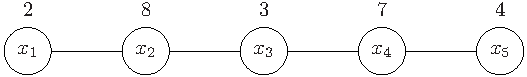
\includegraphics[width=\textwidth]{dp-figs/independent}
\end{frame}


\begin{frame}
  \frametitle{Dynamic Programming Solution}
  \begin{itemize}
  \item Given a set of nodes $\{x_1,\ldots,x_n\}$ with associated weights $\{w_1,\ldots,w_n\}$ we need to find the independent set $S$ such that $\sum_{x\in S}$ is maximum 
\item Assume that the solution $\mathcal{O}$ and the optimal value (which we don't know how to compute yet) is $opt(n)$. The dependence on $n$ comes from the fact that we will express this value in terms of smaller subproblems.
\item Consider the last node $x_n$. Either $x_n$ contributed to $opt(n)$ (i.e. $x_n\in\mathcal{O}$) or not.
\item In the first case $x_n\in\mathcal{O}$ implies that $x_{n-1}\notin\mathcal{O}$. If we can compute the optimal value for $\{x_1,\ldots,x_{n-2}\}$ then we add to it $w_n$ to obtain the optimal value
\item In the second case $x_n\notin\mathcal{O}$ then the optimal value is the same as the one obtained for $\{x_1,\ldots,x_{n-1}\}$
  \end{itemize}
\end{frame}


\begin{frame}
  \frametitle{Dynamic Programming Solution}
  \begin{itemize}
  \item From the analysis above we conclude that 
  \begin{align*}
    opt(n)=\max\left\{\begin{aligned}w_n+opt(n-2)\\opt(n-1) \end{aligned}  \right.
  \end{align*}
\item Applying the above recursive formula to the previous example while noting that $opt[0]=0,opt[1]=2$ (only $x_1$ is included) we get
  \begin{align*}
    opt[5]=\max\left\{\begin{aligned}4+opt[3]\\opt[4] \end{aligned}  \right.
  \end{align*}
  \end{itemize}
\end{frame}

\begin{frame}
    \begin{align*}
    opt[4]=\max\left\{\begin{aligned}7+opt[2]\\opt[3] \end{aligned}  \right. \\
    opt[3]=\max\left\{\begin{aligned}3+opt[1]\\opt[2] \end{aligned}  \right. \\
    opt[2]=\max\left\{\begin{aligned}8+opt[0]\\opt[1] \end{aligned}  \right. 
  \end{align*}
  \begin{itemize}
  \item Since $opt[0]=0$ and $opt[1]=2$ then $opt[2]=8$, $opt[3]=8$,$opt[4]=15$,$opt[5]=15$
  \end{itemize}
\end{frame}

\begin{frame}
  \frametitle{Finding the solution}
  \begin{itemize}
  \item Our method allowed us to compute the optimal value. What if we want the list of vertices for the optimal solution?
  \item In all dynamic programming problems the way to find the optimal solution from the optimal value is almost the same:walk backwards.
  \item In the example above: we start with $x_5$ is it in the solution?
 \item Since $opt[5]=15$ and $opt[4]=15$ then $x_5$ was \textbf{not} selected in the solution
 \item Since $opt[4]=15$ and $opt[3]=8$ then $x_4$ \textbf{was}  selected in the solution, which means $x_3$ cannot be in the solution
 \item Since $opt[2]=18$ and $opt[1]=2$ then $x_2$ \textbf{ was} selected in the solution which means $x_1$ cannot be in the solution
\item from the above the optimal solution includes $\{x_2,x_4\}$.

  \end{itemize}
\end{frame}

\begin{frame}
  \frametitle{Bottom up solution}
  \begin{itemize}
  \item A quick look at the recursive solution we can see that the values of $opt[2]$ and $opt[3]$ were needed twice (for the computation of $opt[3],opt[4],opt[5]$).
  \item If the size of the problem was bigger then these values (among others) would have been needed even more.
  \item In fact this \textbf{top down} approach will lead to exponential complexity because many of the values have to be repeatedly computed.
 \item To avoid this exponential blowup we either have to use memoization (saving the computed values for later use) or solve the problem in a \textbf{ bottom up} manner by using iteration.
  \end{itemize}
\end{frame}
\begin{frame}
  \frametitle{Iterative Solution}
  \begin{itemize}
  \item The iterative solution for the independent set (linear) problem can be written as
\end{itemize}


\begin{center}
  \begin{algorithm}[H]
 
  \DontPrintSemicolon
  \SetKwFunction{IS}{IS}
  \IS{$G$}
  \BlankLine

$opt[0]=0$\;
$opt[1]=w_1$\;
%\tcc{}
\For{$2=1$ \KwTo $n$}{
   $opt[i]=max(opt[i-1],w[i]+opt[i-2])$\;
}

\Return $opt[n]$\;  
\end{algorithm}

  
 \end{center}
 \end{frame}
\section{Weighted Interval Scheduling}

\begin{frame}
  \frametitle{Weighted Interval Scheduling}
  \begin{itemize}
  \item The weighted interval scheduling is a generalization of the interval scheduling we studied using greedy approach.
  \item In the greedy approach the intervals were considered to be equivalent.
  \item In this generalization each interval $i$ has a weight $v_i$ in addition to starting $e(i)$ and ending $f(i)$ time.
  \item A simple example shows that the greedy approach no longer works when the intervals have weights
  \end{itemize}
\end{frame}

\begin{frame}
  \frametitle{Dyanmic Programming Solution}
  
  \begin{itemize}
  \item Let $I$ be a set of intervals where each interval $i$ starts at $e(i)$, ends at $f(i)$ and has values $v(i)$.
  \item Our goal is to find a subset of non-overlapping intervals  $S\subseteq I$ such that $V=\sum_{i\in S}v(i)$ is maximum.
   \item First we sort the intervals by ending time as we did in the case of greedy approach.
  \item Given interval $i$ let $p(i)$ be the largest index $k<i$ such that intervals $k$ and $i$ do not overlap.
  \item As an example let $I=\{(1,2,2),(1,5,7),(4,7,3),(6,8)\}$ where $(a,b,c)$ denotes an interval that starts at $a$, ends at $b$ and has value $c$.
  \item The greedy approach will select the smallest ending time first so the greedy solution gives 
    \begin{align*}
      S=\{(1,2,2),(4,7,3)\}\text{ for a value of } 5
    \end{align*}
\end{itemize}
\end{frame}

\begin{frame}
\begin{itemize}
\item Whereas the optimal solution  is
  \begin{align*}
      S=\{(1,5,7),(6,8,4)\}\text{ for a value of } 11
  \end{align*}
\item The function $p$ in this example has the following values
  \begin{align*}
    p(1)=0\\
    p(2)=0\\
   p(3)=1\\
   p(4)=2\\
  \end{align*}

\item For the general problem where $I=\{i_1,\ldots,i_n\}$ let $opt(n)$ be the optimal solution and consider the last interval $i_n$. 
\end{itemize}
\end{frame}

\begin{frame}
\begin{itemize}
\item There are two cases
  \begin{enumerate}
  \item $i_n\in opt(n)$. In this case all the intervals $i_{p(n)+1},\ldots,i_{n-1}$ overlap with $i_n$ and therefore cannot be in $opt(n)$
  \item $i_n\notin opt(n)$. In this case the solution with $n$ intervals is the same as the solution for $n-1$ intervals since we know $i_n\notin opt$
  \item Since we don't know which case we have, we take the larger one. This means that we compute both possibilities and the larger of the two values is chosen as the optimal solution
  \end{enumerate}

  % \begin{align*}
  %   opt(n)=\max\left\{\begin{aligned}&v_n+opt(p(n))&\text{ case }  i_n\in opt(n)\\&opt(n-1)&\text{ case }i_n\notin opt(n) \end{aligned}  \right.
  % \end{align*}
  \begin{align*}
    opt(n)=\max\begin{dcases} v_n+opt(p(n)) &\text{ if }i_n\in opt(n)\\ opt(n-1) &\text{ if } i_n\notin opt(n)\end{dcases}
  \end{align*}
\item The above is a recursive equation that will allow us to compute the optimal value.
\item If we use the equation as it is it might lead to exponential blow up.
\item Instead we do the computation bottom up
  \end{itemize}
\end{frame}

\begin{frame}
  \begin{algorithm}[H]
 
  \DontPrintSemicolon
  \SetKwFunction{OPT}{OPT}
  \OPT{$I$}
  \BlankLine

$opt[0]=0$\;
%\tcc{}
\For{$i=1$ \KwTo $n$}{
   $opt[i]=max(opt[i-1],v[i]+opt[p[i]])$\;
}

\Return $opt[n]$\;  
\end{algorithm}
\begin{itemize}
\item Clearly the complexity of the above algorithm is $\Theta(n)$.
\item Also we need to sort the intervals by ending time which is $\Theta(n\log n)$.
\item Once the intervals are sorted computing the $p[i]$'s can be done in $\Theta(\log n)$ for each $i$ (similar to binary search) for a total of $\Theta(n\log n)$
\end{itemize}
\end{frame}

\section{Maximum Subarray Sum}
\begin{frame}
  \frametitle{Max subarray sum}
  \begin{itemize}
  \item Recall: given an array of numbers $A_0,A_1,\ldots, A_{n-1}$ let
    \begin{displaymath}
 S_{ij}=\sum_{k=i}^{j}A_k
\end{displaymath}
\item Goal: find $\max_{ij}S_{ij}$
\item Brute force (see first lecture): $\Theta(n^3)$
\item Divide and conquer (see first lecture): $\Theta(n\log n)$
\item Can we do better? yes.
  \end{itemize}
\end{frame}

\begin{frame}
  \frametitle{Dyanmic programming solution}
  \begin{itemize}
  \item Let $M_j=\max_{i}S_{ij}$. $M_j$ is the maximum sum \textbf{ending} at $j$ for all possible values of $0\le i\le j$.(see next slide for details)
\item The max subsequence sum can be written as $\max_{j}M_j$.
\item The key idea is that the values $M_j$ can be stored in an array and computed in $\Theta(n)$ time.
\item What is the relationship between the different values of $M_j$?
\item It is clear that if $M_{j-1}>0$ then $M_j=M_{j-1}+A[j]$.
\item Otherwise $M_{j-1}\le0$ then $M_j=A[j]$
\item The above two cases can be combined to obtain 
  \begin{align*}
    M_j=max(A[j],M_{j-1}+A[j])
  \end{align*}
  \end{itemize}
\end{frame}
\begin{frame}
  \begin{align*}
    M&=\max_j\max_i\sum_{k=i}^jA[k]=\max_j\left(\max_i\sum_{k=i}^jA[k]\right)\\
    &=\max_j M_j
  \end{align*}
  \begin{itemize}
    \item Now
  \end{itemize}
  \begin{align*}
    M_j&=\max_i\sum_{k=i}^jA[k]=\max(\sum_{k=1}^jA[k],\sum_{k=2}^jA[k],\ldots, A[j])\\
    &=\max(\sum_{k=1}^{j-1}A[k]+A[j],\sum_{k=2}^{j-1}A[k]+A[j],\ldots, A[j])
  \end{align*}
\end{frame}
\begin{frame}
  \begin{align*}
    &=\max\left(\sum_{i=1}^{j-1}A[k],\sum_{i=2}^{j-1}A[k],\ldots,0\right)+A[j]\\
    &=\max(M_{j-1}+A[j],A[j])
  \end{align*}
\end{frame}


\begin{frame}
  \frametitle{Example}
  \begin{itemize}
  \item Consider the array
    \begin{align*}
      \left[2,-4,6,3,-7,4,5,-5,-6,4,6,-4,3 \right]
    \end{align*}
\item One can guess by inspection that the subarray $\left[6,3,-7,4,5 \right]$ will give the largest sum.
\item using the proposed algorithm we get
  \begin{align*}
    \left[2,-2,6,9,2,6,11,6,0,4,10,6,9 \right]
  \end{align*}
\item By scanning the result we obtain the maximum 11 as it should be.
\item Note that this method not only computes the result for $n=13$ elements but also solves \textbf{all subproblems}
  \end{itemize}
\end{frame}

\begin{frame}
  \frametitle{Code}
\begin{algorithm}[H]
 
  \DontPrintSemicolon
  \SetKwFunction{MaxSubarraySum}{MaxSubarraySum}
  \MaxSubarraySum{$A$}
  \BlankLine

$M[0]\gets 0$\;
$max\gets 0$\;

\For{$i=1$ \KwTo $n$}{
   $M[i]\gets max(A[i],A[i]+M[i-1])$\;
}
\tcc{Now compute the maximum of all sums}
\For{$i=1$ \KwTo $n$}{
  \If{$M[i]>max$}
   {
     $max\gets M[i]$\;
    }
}
\Return $max$\;  
\end{algorithm}
    
\end{frame}

\section{Maximum Common Subsequence}
\begin{frame}
  \frametitle{Maximum Common Subsequence}
  \begin{itemize}
  \item Consider two strings $X$ and $Y$. Our goal is to find the longest sequence that is contained in both $X$ and $Y$.
  
  \item For example: $BDBDC$ and $ADBC$ then the longest common sequence is $DBC$
  \item Note that the characters in the sequence do not have to be necessarily consecutive
  \item This problem is \textbf{different} from the \textbf{common substring} problem where the characters in the common sequence are required to be consecutive.
  \item In this example the longest common substring is $DB$
  \end{itemize}
\end{frame}

\begin{frame}
  \frametitle{Dynamic Programming Solution}
  \begin{itemize}
  \item Consider two strings $X=x_1x_2\ldots x_{n-1}x_n$ and $Y=y_1y2\ldots y_{m-1}y_m$. We denote the prefix of length $k$ of $X$ by $X_k=x_1\ldots x_k$  so that $X=X_n$ and $Y=Y_m$.
\item  let $LCS(X,Y)$ be the \textbf{length} of the longest common subsequence between $X$ and $Y$ then we can write $LCS(X,Y)=LCS(X_n,Y_m)$.
  \item If $x_n=y_m$ then the common subsequence must include $x_n$. In this case $LCS(X_n,Y_m)=LCS(X_{n-1},Y_{m-1})+1$ .
  \item If $x_n\neq y_m$ then $LCS(X_n,Y_m)=\max (LCS(X_n,Y_{m-1}),LCS(X_{n-1},Y_m))$
  \end{itemize}
\end{frame}

\begin{frame}
  \frametitle{Bottom up algorithm}
  \begin{itemize}
  \item First we note that if one substring has 0 elements the length of the common subsequence is 0. Therefore $LCS[i][0]=0$ and $LCS[0][j]=0$ for all $i,j$
  \end{itemize}

\begin{algorithm}[H]
 
  \DontPrintSemicolon
  \SetKwFunction{LCS}{LCS}
  \LCS{$X$,$Y$}
  \BlankLine

\For{$i=1$ \KwTo $n$}{
\For{$j=1$ \KwTo $m$}{
 \If{$X[i]=X[j]$}{
   $LCS[i][j] \gets 1+LCS[i-1][j-1]$\;
}
\Else {
   $LCS[i][j]\gets max(LCS[i-1][j],LCS[i][j-1])$\;
}
}
}

\Return $LCS[n][m]$\;  
\end{algorithm}
\end{frame}
\begin{frame}
  \frametitle{Example}
  Consider the two strings $X=ABCD$ and $Y=AABDC$
\end{frame}
\section{Knapsack}
\begin{frame}
  \frametitle{Knapsack}
  
  \begin{itemize}
  \item Given a knapsack of capacity $W$ and $n$ items $x_1,\ldots ,x_n$ with weights $w_1,\ldots,w_n$ and values $v_1,\ldots,v_n$ we need to find a subset $S\subseteq\{x_1,\ldots,x_n\}$ such that
    \begin{align*}
      &\sum_{x_i\in S}w_i\le W \\
      &\sum_{x_i\in S}v_i\text{ is maximum}  \\
    \end{align*}
  \end{itemize}
\end{frame}

\begin{frame}
  \frametitle{Dynamic Programming }
  \begin{itemize}
  \item Let $S_n$ be the optimal solution when the problem contains $n$ items and consider item $x_n$. There are two possibilities:
  \item Either $x_n\in S_n$. Suppose that we know $S_{n-1}$ the optimal solution for the subproblem including the first $n-1$ items. Can one add to that solution $x_n$?No, because when the weight of $x_n$ is added, the total weight might be greater than $W$. Instead we look for the optimal solution for the first $n-1$ items with a knapsack of capacity $W-w_n$ to leave room for item $x_n$. Therefore $S_n(W)=v_n+S_{n-1}(W-w_n)$
  \item Or $x_n\notin S_n$. Since $x_n\notin S_n$ then we don't need to leave room for it when we compute $S_{n-1}$. In this case $S_n(W)=S_n(W)$
  \end{itemize}
\end{frame}

\begin{frame}
  \begin{itemize}
  \item Because we don't know apriori if $x_n\in S_n$ we compute both values and take the largest.


    \begin{align*}
      S(n,W)=\max\left\{ \begin{aligned}v_n+S(n-1,W-w_n)\\S(n-1,W)\end{aligned}\right.
    \end{align*}
\item Before writing a bottom up solution we need to take care of the boundary conditions.
\item Anytime the capacity of the knapsack $W=0$ the solution is just $0$.
\item Also we need to take int account the case when $w_n> W$. In this case $S(n,W)=S(n-1,W)$
  \end{itemize}
\end{frame}

\begin{frame}
  
\begin{algorithm}[H]
   \DontPrintSemicolon
  \SetKwFunction{Knapsack}{Knapsack}
  \Knapsack{$w$,$v$,$W$}
  \BlankLine
\tcc{if $W=0$ then solution for any}
\tcc{ number of items is 0}
\For{$i=1$ \KwTo $n$}{
   S[i][0]=0
}
\tcc{for any $W$ zero items gives 0}
\For{$i=1$ \KwTo $W$}{
   S[0][i]=0
}
\tcc{Now the solution}
\For{$j=1$ \KwTo $W$}{
\For{$i=1$ \KwTo $n$}{
   $S[i][j]$=$\max \left(S[i-1][j],v[i]+S[i-1][j-w[i]]\right)$
}
}
\end{algorithm}
\end{frame}


\begin{frame}
  \frametitle{Example}
  Consider the following instance of the knapsack problem where the knapsack size is $W=13$.
  \begin{center}
    \begin{tabular}{|c|c|c|}
      \hline
      $v_1=2$ & $w_1=3$ & $\frac{v_1}{w_1}=0.66$\\
      $v_2=4$ & $w_2=6$ & $\frac{v_2}{w_2}=0.66$\\
      $v_3=5$ & $w_3=7$ & $\frac{v_3}{w_3}=0.71$\\
      $v_4=6$ & $w_4=8$ & $\frac{v_4}{w_4}=7.5$\\
      \hline
    \end{tabular}
  \end{center}
  Note that a greedy approach would choose items $v_4$ and $v_1$ for a total value of 8 
  whereas the optimal is 9 by choosing items 3 and 2.
\end{frame}
\begin{frame}
\begin{tabular}{c|cccccccccccccc}
$n\backslash w $&0 &1 &2 & 3 & 4 & 5 & 6 & 7 & 8 & 9 & 10 & 11 & 12 & 13\\
\hline  
0 &0 & 0 & 0 & 0 & 0 & 0 & 0 & 0 & 0 & 0 & 0 & 0 & 0 & 0  \\
1 &0 & 0 & 0 & 2 & 2 & 2 & 2 & 2 & 2 & 2 & 2 & 2 & 2 & 2  \\
2 &0 & 0 & 0 & 2 & 2 & 2 & \textcircled{4} & 4 & 4 & 6 & 6 & 6 & 6 & 6  \\
3 & 0 & 0 & 0 & 2 & 2 & 2 & 4 & 5 & 5 & 6 & 7 & 7 & 7 & \textcircled{9}  \\
4 &0 & 0 & 0 & 2 & 2 & 2 & 4 & 5 & 6 & 6 & 7 & 8 & 8 & 9  \\
\hline
\end{tabular}
\end{frame}


\section{Subset Sum}
\begin{frame}[fragile]
  \frametitle{Subset sum}
  \begin{itemize}
  \item We are given an array $A$ of $n$ elements and an integer value $S$ and we ask if there is a subset of $A$ whose sum is $S$
  \item We start with the last element. There are two choices
    \begin{enumerate}
    \item Either the last element is in the sum in which case we have to find a subset of of the first $n-1$ elements whose sum is $S-A[n]$
    \item Or the last element is not in the sum in which case we have to find a subset of the first $n-1$ elements whose sum is $S$
    \end{enumerate}
\item The above reasoning will lead to 
  \end{itemize}
\begin{lstlisting}[numbers=none]
subset(A,n,S){
  if(n==0) return false
  if(S==0) return true
  return subset(A,n-1,S)||subset(A,n-1,S-A[n])
\end{lstlisting}
\end{frame}
\begin{frame}[fragile]
  \frametitle{Example}
  \begin{itemize}
  \item Consider the array $A={2,7,3,1}$ and $S=6$.
  \end{itemize}
\begin{verbatim}
subset(A,4,6)=subset(A,3,6)||subset(A,3,5)=false||true
subset(A,3,6)=subset(A,2,6)||subset(A,2,3)=false||false=false
subset(A,3,5)=subset(A,2,5)||subset(A,2,2)=false||true=true
subset(A,2,6)=false
subset(A,2,3)=false
subset(A,2,5)=false
subset(A,2,2)=true
\end{verbatim}
\end{frame}
\begin{frame}
  \frametitle{Bottom up}
  We use the recurrence relation that we have obtained to solve the subsetsum problem in a bottom
  up manner. First note that if the required sum is 0 then the answer is always true. Also if the number
  of elements is 0 then with the exception of sum=0 all the answers should be false.
  
\end{frame}
\begin{frame}
  
\begin{algorithm}[H]
  \DontPrintSemicolon
 \SetKwFunction{SubsetSum}{SS}
 \SubsetSum{$A$,$S$}
 \BlankLine
\tcc{if $S=0$ then solution for any}
\tcc{ number of items is True}
\For{$i=0$ \KwTo $n$}{
  R[i][0]=True
}
\tcc{for any $S$ other than zero }
\tcc{0 items is False}
\For{$j=1$ \KwTo $S$}{
  R[0][j]=False
}
\tcc{Now the solution}
\For{$i=1$ \KwTo $n$}{
\For{$j=1$ \KwTo $S$}{
  $R[i][j]$=$R[i-1][j]$ or $R[i-1][j-A[i]]$
}
}
\end{algorithm}
\end{frame}
\section{Balanced Partition}
\begin{frame}
  \frametitle{Balanced Partition of a Set}
  \begin{itemize}
  \item Suppose that you have a set of $n$ integers $A=\{A_1,\ldots, A_n\}$.
  \item Let $S_1$ and $S_2$ be a partition of $A$ i.e. $S_1\cup S_2=A$ and $S_1\cap S_2=\emptyset$.
 \item Let $sum_1=\sum_{a\in S_1}a$ and $sum_2=\sum_{a\in S_2}$ be the sum of elements in each partition.
 \item Our goal is to find $S_1$ and $S_2$ such that $\abs{sum_1-sum_2}$ is minimum.
  \end{itemize}
\end{frame}

\begin{frame}
  \begin{itemize}
  \item Let $\sigma=\sum_{a\in A}a$, i.e.  the sum of all elements in $A$.
  \item Given $A$ we know how to find if there is a subset of $A$ whose sum is $k$.
  \item Let $p(i,j)$ be true if the first $i$ elements of $A$ have a subset whose sum is $j$.
  \item This is the subset sum problem we have studied previously.
  \item Computer $p(i,j)$ for all $1\le i\le n$ and $0\le j\le \sigma/2$.
  \item then consider the set
    \begin{align*}
      \{ \abs{j-\sigma/2}\mid p(n,j)=1  \}
    \end{align*}
\item Our answer is 
  \begin{align*}
    \min_j\{ \abs{j-\sigma/2}\mid p(n,j)=1  \}
  \end{align*}
  \end{itemize}
\end{frame}
\begin{frame}
  \frametitle{Example}
  Consider the set =$\{1,6,11\}$ whose sum is 18 so $\sigma/2=9$. We compute the subset
  sum problem in a bottom up fashion we get
  % \begin{center}
  %   \begin{tabular}{c|cccccccccc}
  %   - & 0 & 1 &2 &3 &4 &5 & 6 & 7 & 8 & 9 
  %   \end{tabula}
  % \end{center}
\end{frame}
\section{Sequence Alignment}
\begin{frame}
  \frametitle{Sequence Alignment}
  

\begin{itemize}
\item For example
  \begin{align*}
    &ACTGG\!-\!ATT\\
    &ACGGGTATG
  \end{align*}
\item We need to align two sequence to minimize the "cost". 
\item Cost the sum of costs where each dash incurs a cost $\alpha_{gap}$ and cost of mismatch $\alpha$. 
\item Note that we are assuming that all mismatches are the same cost even though it is easy to modify the cost to depend on the type of mismatch
\end{itemize}
\end{frame}
\begin{frame}
  \begin{itemize}
  \item Given strings $X=x_1\ldots x_n$ and $Y=y_1\ldots y_m$ we need to find the "best" alignment: the one that leads to the smallest cost
  \item Let $X_i$ be the prefix of $X$ of size $i$, i.e. $X_i=x_1\ldots x_i$.
  \item Let $opt(X_n,Y_m)$ be the optimal solution for prefixes $X_n=X$ and $Y_m=Y$. We can write
    \begin{align*}
      opt(X_n,Y_m)=\min
    \begin{cases}
     \alpha+ opt(X_{n-1},Y_{m-1})\\
     \alpha_{gap}+ opt(X_{n-1},Y_m)\\
     \alpha_{gap}+ opt(X_{n},Y_{m-1})\\
   \end{cases}
    \end{align*}
  \end{itemize}
\end{frame}
\begin{frame}
  \frametitle{Base cases}
  \begin{itemize}
  \item Before we implement the algorithm we need to determine the value of the base cases: $opt(X_i,0)$ and $opt(0,Y_i)$.
  \item Note that when one string is empty we need $i$ gaps to match the other so
  \item $opt(X_i,0)=opt(0,Y_i)=i\cdot\alpha_{gap}$
  \end{itemize}
\end{frame}

\begin{frame}
  \frametitle{Example}
  Consider the two strings $X="CG"$ and $Y="CA"$ with the cost of a gap $\alpha_g$=3 and cost of mismatch $\alpha=7$.
  The solution obtained from the table below is $CG-$ and $C-A$.
  \center
  \begin{tabular}{|c|ccc|}
    \hline
    X$\backslash$ Y & "" & C & CA \\
    \hline
    "" & 0 & 3 & 6\\
    C  & 3 & $\nwarrow 0$ & 3\\
    CG & 6 & $\uparrow3 $ & $\leftarrow 6$\\
    \hline
  \end{tabular}
\end{frame}
\section{Shortest Path}

\begin{frame}
  \frametitle{Bellman-Ford Single Source}
  \begin{itemize}
  \item The Bellman-Ford algorithm uses dynamic programming to compute the shortest path in graph $G=\left<V,E\right>$
  \item The quantity to be optimized is the shortest distance using \textit{at most $i$ edges}.
  \item Let $d[u,i]$ be the shortest path distance from some source $s$ to destination $u$ using \textit{at most} $i$ edges.
\item Let $c_{v,u}$ be the cost of edge $(v,u)\in E$ or $\infty$ otherise.
  \item Then $d[u,i+1]$ can be written as 
    \begin{align*}
      d[u,i+1]=\min (d[u,i],\min_{v\in V}(d[v,i]+c_{v,u}))
    \end{align*}
  \end{itemize}
\end{frame}

\begin{frame}
  \frametitle{Example}
  In the graph below we would lile to use the Bellman-Ford algorithm
  to compute the shortest path from node $a$ to all other nodes.
  \begin{figure}[h]
    \centering
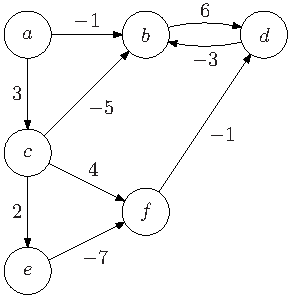
\includegraphics[width=0.4\textwidth]{dp-figs/bellman-ford}
  \end{figure}
\end{frame}
\begin{frame}
  \begin{tabular}[h]{c|cccccc}
    &0 & 1& 2 & 3 & 4 &5\\
   \hline
   a&    0&0&0&0&0&0\\
   b& $\infty$ &-1&-2&-2&-2&-6\\
   c& $\infty$ &3&3&3&3&3\\
   d& $\infty$ & $\infty$ &5&4&-3&-3\\
   e& $\infty$ & $\infty$ &5&5&5&5\\
   f& $\infty$ & $\infty$ &7&-2&-2&-2
     \end{tabular}
\end{frame}
\begin{frame}[fragile]
  \frametitle{Implementation}
  \begin{itemize}
  \item Encoding the edge weights
\begin{verbatim}
0-1:-1
0-2:3
1-3:6
2-1:-5
2-4:2
2-5:4
3-1:-3
4-5:-7
5-3:-1
\end{verbatim}
  \item We choose a large value compared to the edge weights in the graph, say 100.
  \end{itemize}

\end{frame}
\begin{frame}
\frametitle{Solution for the example}
  \begin{tabular}[h]{c|cccccc}
 &0 & 1& 2 & 3 & 4 &5\\
\hline
a&    0&0&0&0&0&0\\
b&100&-1&-2&-2&-2&-6\\
c&100&3&3&3&3&3\\
d&100&99&5&4&-3&-3\\
e&100&100&5&5&5&5\\
f&100&93&7&-2&-2&-2
  \end{tabular}
\end{frame}
\begin{frame}[fragile]
\begin{lstlisting}
import numpy as np
num=6
opt=np.full((num,num),100)
opt[0,0]=0
edge=np.full((num,num),100)

f=open("graph1.txt","r")
input=f.read()
lines=input.splitlines()
for line in lines:
  x=line.split(":")
  cost=x[1]
  y=x[0].split("-")
  s=y[0]
  d=y[1]
  edge[int(s),int(d)]=int(cost)
\end{lstlisting}
\end{frame}
\begin{frame}[fragile]
\begin{lstlisting}
pred=np.full(num,-1)
for l in range(1,num): #iterate over length
  for n in range(0,num): #iterate over nodes
    opt[n,l]=opt[n,l-1]
    for m in range(0,num):#iterate over neighbors
      s=opt[m,l-1]+edge[m,n]
      if s<opt[n,l]:
        opt[n,l]=s
        pred[n]=m
\end{lstlisting}
\end{frame}
\end{document}

%%% Local Variables: 
%%% mode: late
%%% TeX-master: t
%%%
